\documentclass[a4paper,twoside,11pt]{article}

\usepackage[a4paper, total={17cm, 24cm}]{geometry}
% generated by Docutils <http://docutils.sourceforge.net/>
\usepackage{cmap} % fix search and cut-and-paste in Acrobat
\usepackage{ifthen}
\usepackage[T1]{fontenc}
\usepackage[utf8]{inputenc}
\setcounter{secnumdepth}{3}
\usepackage{longtable,ltcaption,array}
\setlength{\extrarowheight}{2pt}
\newlength{\DUtablewidth} % internal use in tables

\usepackage[parfill]{parskip}

%%% Custom LaTeX preamble
% PDF Standard Fonts
\usepackage{mathptmx} % Times
\usepackage[scaled=.90]{helvet}
\usepackage{courier}
\usepackage{graphicx}
\graphicspath{{images/}}
\usepackage{alltt}
\usepackage{float}
\usepackage{listings}
\lstloadlanguages{csh, python}
\usepackage{pdfpages}

%%% MICADO PDR doc packages
\usepackage{dmd-doc}
\usepackage[english]{babel}
\usepackage{lastpage}
\usepackage{multirow}
\usepackage{supertabular}
\usepackage{fancyhdr}
\usepackage{amsmath}
\usepackage{color}
\definecolor{darkblue}{rgb}{0, 0, 0.5}
\definecolor{listingbg}{gray}{0.95}


%%% User specified packages and stylesheets


%%%%%%%%%%%%%%%%%%%%%%%%%%%%%%%%%%%%%%%%%%%%%%%%%%%%%%%%%%%%%%%%%%%%%%%%%%%%%%%%%
% Docutils-specific commands
%%%%%%%%%%%%%%%%%%%%%%%%%%%%%%%%%%%%%%%%%%%%%%%%%%%%%%%%%%%%%%%%%%%%%%%%%%%%%%%%%


% admonition (specially marked topic)
\providecommand{\DUadmonition}[2][class-arg]{%
  % try \DUadmonition#1{#2}:
  \ifcsname DUadmonition#1\endcsname%
    \csname DUadmonition#1\endcsname{#2}%
  \else
    \begin{center}
      \fbox{\parbox{0.9\linewidth}{#2}}
    \end{center}
  \fi
}

% class handling for environments (block-level elements)
% \begin{DUclass}{spam} tries \DUCLASSspam and
% \end{DUclass}{spam} tries \endDUCLASSspam
\ifx\DUclass\undefined % poor man's "provideenvironment"
 \newenvironment{DUclass}[1]%
  {\def\DocutilsClassFunctionName{DUCLASS#1}% arg cannot be used in end-part of environment.
     \csname \DocutilsClassFunctionName \endcsname}%
  {\csname end\DocutilsClassFunctionName \endcsname}%
\fi

% subtitle (in document title)
\providecommand*{\DUdocumentsubtitle}[1]{{\large #1}}

% title for topics, admonitions, unsupported section levels, and sidebar
\providecommand*{\DUtitle}[2][class-arg]{%
  % call \DUtitle#1{#2} if it exists:
  \ifcsname DUtitle#1\endcsname%
    \csname DUtitle#1\endcsname{#2}%
  \else
    \smallskip\noindent\textbf{#2}\smallskip%
  \fi
}

% hyperlinks:
\ifthenelse{\isundefined{\hypersetup}}{
  \usepackage[colorlinks=true,linkcolor=blue,urlcolor=blue]{hyperref}
  \usepackage{bookmark}
  \urlstyle{same} % normal text font (alternatives: tt, rm, sf)
}{}
\hypersetup{
  pdftitle={SimCADO v2 User Manual},
}


%%%%%%%%%%%%%%%%%%%%%%%%%%%%%%%%%%%%%%%%%%%%%%%%%%%%%%%%%%%%%%%%%%%%%%%%%%%%%%%%%
% Set title values
%%%%%%%%%%%%%%%%%%%%%%%%%%%%%%%%%%%%%%%%%%%%%%%%%%%%%%%%%%%%%%%%%%%%%%%%%%%%%%%%%

\dmdTitle{SimCADO v2 User Manual}
\dmdDocId{ELT-TRE-MCD-56306-0058}
\dmdIssue{1.0}
\dmdDate{12. April 2021}
\dmdPreparedBy{K. Leschinski}
\dmdPreparedOn{2021-04-12}
\dmdPreparedSig{\resizebox{2.5cm}{!}{
\includegraphics{scribble}}}
\dmdApprovedBy{}
\dmdApprovedOn{}
\dmdApprovedSig{}
\dmdReleasedBy{}
\dmdReleasedOn{}
\dmdReleasedSig{}


%%%%%%%%%%%%%%%%%%%%%%%%%%%%%%%%%%%%%%%%%%%%%%%%%%%%%%%%%%%%%%%%%%%%%%%%%%%%%%%%%
% Body
%%%%%%%%%%%%%%%%%%%%%%%%%%%%%%%%%%%%%%%%%%%%%%%%%%%%%%%%%%%%%%%%%%%%%%%%%%%%%%%%%

%%% Body
\begin{document}

% listings style
\lstset{basicstyle=\ttfamily,
        columns=flexible,
        frame=single,
        backgroundcolor=\color{listingbg},
        captionpos=b,
        showspaces=false}

\dmdmaketitle

%\emptypage{This page was intentionally left blank}

\begin{center}
  \textbf{Change record}

  \tablehead{\hline
    \multicolumn{1}{|c|}{Issue/Rev.} &
    \multicolumn{1}{|c|}{Date} &
    \multicolumn{1}{|c|}{Section/Parag.\ affected} &
    \multicolumn{1}{|c|}{Reason/Initiation/Documents/Remarks} \\
    \hline}
  \tabletail{\hline}

  \begin{supertabular}{|l|l|l|l|}
   0.0.1 & 2020-10-15 & All & Layout initialised \\
   1.0.0 & 2021-03-22 & All & Finished initial release version \\
   \hline
  \end{supertabular}

\end{center}

%\emptypage{This page was unintentionally left blank}

\setcounter{tocdepth}{3}
\tableofcontents
% \cleardoublepage



\section*{Abbreviations}
\label{sec:abbreviations}

%\tablehead{%
%  \hline
%  \multicolumn{1}{|c|}{Abbreviation} &
%  \multicolumn{1}{|c|}{Meaning} \\
%  \hline}
%\tabletail{\hline}

\tablehead{}
\tabletail{}
\begin{supertabular}{ll}
  DFS & Data Flow System \\
  ELT & Extremely Large Telescope \\
  ESO & European Southern Observatory \\
  HCI & High Contrast Imaging \\
  IMG & Imaging observing modi \\
  MCAO & Multi-Conjugate Adaptive Optics \\
  PSF & Point Spread Function \\
  SCAO & Single Conjugate Adaptive Optics \\
  SPEC & Spectroscopy observing modi \\
  TBC & To Be Confirmed \\
  TBD & To Be Decided \\
\end{supertabular}


\section{Scope}
\label{sec:introduction}

This document aims to introduce the reader to the ScopeSim instrument simulator and the MICADO instrument packages that have been developed as part of the MICADO instrument simulator work package.
ScopeSim is a second generation instrument simulation environment, following on from the original SimCADO package.
In this context, the title of the document "SimCADO v2 user manual" refers to the fact that the MICADO instrument simulator is now a combination of the ScopeSim software and the associated MICADO packages.
The ScopeSim environment consists of a series of Python packages, with the ScopeSim instrument simulation engine at its core.
All packages are available within the standard python ecosystem.
The ScopeSim ecosystem maintains a very strict split between code and data.
The simulation engine and all associated software packages are completely instrument agnostic.
Instrument models can only be initialised by passing an instrument specific data package to the ScopeSim engine.

For MICADO two instrument data package were produced as input for the ScopeSim engine: ``MICADO'' and ``MICADO\_Sci''.
The original use case for the simulator was as a means of producing raw detector frames to aid in the development of the MICADO data reduction pipeline.
Hence the ``MICADO`` instrument data package contains all the elements needed to simulate realistic raw detector readout images.
The primary audience for the ``MICADO`` instrument data package is the MICADO dataflow system work package.
Many of the effect included in the ``MICADO`` package will be removed by the data reduction pipeline.
Simulating and subsequently removing these effects results in a substantial amount of redundant computational overhead for the second group of use cases for the software: science case feasibility studies.
In order to enable rapid iteration of simulations for these feasibility studies, a second instrument data package was compiled: ``MICADO\_Sci``.
``MICADO\_Sci`` contains only the optical effects that will remain in the images after the data reduction pipeline has successfully processed the images.

This document should be seen as the initial introduction to ScopeSim and the MICADO data packages.
It contains the following information:
\begin{itemize}
\item Introduction to ScopeSim environment
\item Where to find the online documentation
\item How to begin simulating MICADO observations with ScopeSim
\item How to control simulations
\item Building on-sky target object as input for ScopeSim
\item Five use case examples for the imaging and spectroscopy modes of MICADO
\end{itemize}

It should be noted that what is contained in this document is a subset of what is available in the online documentation for ScopeSim.
More examples and information are available at \url{https://scopesim.readthedocs.io/}.


\section{Applicable and Reference Documents}
\label{sec:documents}

\subsection{Applicable Documents}

\begin{center}
  \tablehead{\hline
    \multicolumn{1}{|c|}{Nr} &
    \multicolumn{1}{|c|}{Doc.\ Nr} &
    \multicolumn{1}{|c|}{Doc.\ Title} &
    \multicolumn{1}{|c|}{Issue} &
    \multicolumn{1}{|c|}{Date} \\
    \hline}
  \tabletail{\hline}

  \begin{supertabular}{|l|l|l|c|l|}
    AD\,1 & ELT-ICD-MCD-56306-0058 & SimCADO User Manual & 1.0 & 2021-04-12 \\
    AD\,2 & ELT-ICD-MCD-56306-0059 & Instrument data packages for the & & \\
    & & MICADO simulation environment & 1.0 & 2021-04-12 \\
    AD\,3 & ELT-ICD-MCD-56306-0060 & ScopeSim - A modular astronomical & & \\
    & & instrument data simulation environment & 1.0 & 2021-04-12 \\
    AD\,4 & ELT-TRE-MCD-56300-0014 & MICADO Masks, Stops, and Filters Description & 2.9 & 2020-12-04 \\
  \end{supertabular}
\end{center}

\subsection{Reference Documents}

\begin{center}
  \tablehead{\hline
    \multicolumn{1}{|c|}{Nr} &
    \multicolumn{1}{|c|}{Doc.\ Nr} &
    \multicolumn{1}{|c|}{Doc.\ Title} &
    \multicolumn{1}{|c|}{Issue} &
    \multicolumn{1}{|c|}{Date} \\
    \hline}
  \tabletail{\hline}

  \begin{supertabular}{|l|l|l|c|l|}
    \hline
    RD\,1 & ELT-PLA-MCD-56301-0004 & Operational Concept Description &
    2 & 2019-11-09 \\
    RD\,2 & ELT-TRE-MCD-56300-0011 & MICADO System Design and Analysis & 1.5 &
    2021-04-12 \\
    RD\,3 & ELT-ICD-MCD-56306-0050 & SimCADO: the Data Simulator for MICADO & 1.0 & 2018-09-27 \\

  \end{supertabular}
\end{center}



\section{Introduction%
  \label{introduction}%
}


\subsection{An overview of the ScopeSim environment%
  \label{an-overview-of-the-scopesim-environment}%
}

ScopeSim is a modular and flexible suite of python packages that enable (almost) any astronomical optical (observatory/telescope/instrument) system to be simulated.

The suite of packages can be used by a wide audience for a variety of purposes; from a astronomer interested in simulating reduced observational data, to a pipeline developer who needs raw calibration data for testing the pipeline.

\DUadmonition[warning]{
\DUtitle[warning]{Warning}

Add image of scopesim environment
}

ScopeSim achieves this level of flexibility by adhering to strict interfaces between the package, e.g: the ScopeSim engine package is completely instrument and object agnostic.
All information and data relating to any specific optical configuration is kept exclusively in the instrument packages hosted in the instrument reference database (IRDB).
Similarily, the engine has no clue about what it is observing until run-time.
The description of the on-sky source is keep exclusively within the target \texttt{templates} package (see \texttt{scopesim\_templates}).

The core of the ScopeSim environment are the three packages:

\begin{itemize}
\item \texttt{ScopeSim}: the simulation engine

\item \texttt{ScopeSim\_templates}: descriptions of the on-sky sources

\item \texttt{IRDB}: the instrument reference database.
\end{itemize}

In addition to the core package, there are several support packages:

\begin{itemize}
\item \texttt{AnisoCADO}: simulates SCAO PSFs for the ELT

\item \texttt{SkyCalc\_ipy}: queries the ESO skycalc service for atmospheric spectral curves

\item \texttt{SpeXtra}: provides easy access to many well-known spectral libraries

\item \texttt{Pyckles}: a light-weight wrapper for the Pickles (1998) and Brown (2010) catalogues.
\end{itemize}

Each of these packages will be discussed in detail in the remainder of this document.


\subsection{Document Scope%
  \label{document-scope}%
}

This document is not intended to be a comprehensive description of the ScopeSim environment. Rather is aims to introduce the reader to the elements that make up ScopeSim and directs the reader towards the online documentation for each of the packages, should the reader wish to dive deeper into the material.


\subsection{Rationale for the ScopeSim environment%
  \label{rationale-for-the-scopesim-environment}%
}

Until now most instrument consortia have developed their own simulators.
The general argument is that every new instrument is sufficiently different from anything that has been previously developed, that it would make no sense to adapt already existing code.
This statement is true to some extent.
Every new instrument must differ in some way from all existing instruments in order for it to be useful to the astronomical community.
However when looked at from a global perspective, every optical system is comprised primarily of elements common to all other systems.
Atmospheric emission, mirror reflectivities, filter transmission curves, point spread functions, read-out noise, detector linearity, hot pixels, are just a few of the effects and artifacts that every astronomical optical system contains.
Furthermore, while the amplitude and shape of each effect differs between optical systems, there are still commonalities in the way each effect can be described programmatically.

ScopeSim's main goal is to provide a framework for modelling (almost) any astronomical optical system by taking advantage of all these commonalities.
What astropy has done for python landscape in astronomy, ScopeSim aims to do for the instrument simulator landscape.


\subsection{Community involvement%
  \label{community-involvement}%
}

The scopesim environment has been developed as an open source project so that it is possible for others in the astronomical community to be involved in the expansion of both core and perifery functionality.
The interface of both the \texttt{Effect} and \texttt{Source} objects was kept as minimalistic in order to keep the barrier to entry as low as possible.

For the \texttt{ScopeSim\_templates} package we encourage the submission of both basic and detailed custom \texttt{Source} objects for any astronomical source.
The package is designed in such a way as to be highly scalable to accommodate descriptions of the myriad of astronomical objects.

For users who need custom \texttt{Effect} objects for their optical model, there is the possibility of adding \textquotedbl{}plug-in\textquotedbl{} \texttt{Effect} objects at run time.
We however encourage anyone who has made these custom \texttt{Effects} to submit a pull request to the ScopeSim github page, so that we can include these \texttt{Effects} in the next major release.


\subsection{Documentation and code bases%
  \label{documentation-and-code-bases}%
}

\setlength{\DUtablewidth}{\linewidth}
\begin{longtable}[c]{|p{0.315\DUtablewidth}|p{0.315\DUtablewidth}|p{0.315\DUtablewidth}|}
\caption{docs\_and\_code}\\
\hline

Package
 & 
Documentation
 & 
Code base
 \\
\hline

ScopeSim
 & 
\url{https://scopesim.readthedocs.io/}
 & 
\url{https://github.io/astronomyk/scopesim}
 \\
\hline

ScopeSim\_templates
 & 
\url{https://scopesim-templates.readthedocs.io/}
 & 
\url{https://github.com/astronomyk/ScopeSim_templates}
 \\
\hline

IRDB
 & 
\url{https://irdb.readthedocs.io/en/latest/}
 & 
\url{https://github.com/astronomyk/IRDB}
 \\
\hline

AnisoCADO
 & 
\url{https://anisocado.readthedocs.io/}
 & 
\url{https://github.com/astronomyk/AnisoCADO}
 \\
\hline

SkyCalc\_ipy
 & 
\url{https://skycalc-ipy.readthedocs.io/en/latest/}
 & 
\url{https://github.com/astronomyk/SkyCalc_iPy}
 \\
\hline

SpeXtra
 & 
\url{https://spextra.readthedocs.io/en/latest/}
 & 
\url{https://github.com/miguelverdugo/speXtra}
 \\
\hline

Pyckles
 & 
\url{https://pyckles.readthedocs.io/en/latest/}
 & 
\url{https://github.com/astronomyk/Pyckles}
 \\
\hline
\end{longtable}
\label{tbl-list-of-packages}



\section{Online Documentation%
  \label{online-documentation}%
}

\begin{itemize}
\item Where to find what

\item Installing ScopeSim

\item Downloading a package
\end{itemize}



\section{Basic functionality%
  \label{basic-functionality}%
}

A basic simulation of an ELT/MICADO observation using the MICADO\_Sci package would look something like this:

\begin{quote}
\begin{alltt}
\begin{lstlisting}[frame=single]
# Setup everything
import scopesim_templates
from scopesim.server.database import download_package
import scopesim

scopesim.download_package(["locations/Armazones",
                           "telescopes/ELT",
                           "instruments/MICADO_Sci"])

# Make the on-sky target
src = scopesim_templates.basic.stars.cluster()

# Load the model of MICADO and the ELT
cmd = scopesim.UserCommands(use_instrument="MICADO_Sci",
                            properties=\{"!OBS.dit": 60, "!OBS.ndit": 10,
                                        "!INST.filter_name": "Ks"\})
micado = scopesim.OpticalTrain(cmd)

# Run the simulation
micado.observe(src)
micado.readout(filename="my_image.fits")
\end{lstlisting}
\end{alltt}
\end{quote}


\subsection{General Workflow%
  \label{general-workflow}%
}

The general workflow for simulating observations can be seen in the code in the previous section.
There are three (four) major components of any simulation workflow:

\begin{enumerate}
\item the target description,

\item the telescope/instrument model, and

\item the observation.
\end{enumerate}

The zeroth (or fourth) step is the setup stage which include the import statements and the package downloads.

The first step of any simulation run is defining the on-sky target.
This is probably the most time intensive step and requires the user to know what they want to observe.
In the code above we make use of the \href{https://scopesim-templates.readthedocs.io/en/latest/}{ScopeSim\_Templates} package to create a \texttt{Source} object for an open cluster with default values (i.e. 1000 Msun at 50 kpc).:

\begin{quote}
\begin{alltt}
\begin{lstlisting}[frame=single]
src = scopesim_templates.basic.stars.cluster()
\end{lstlisting}
\end{alltt}
\end{quote}

\texttt{Source} objects are discussed in a later chapter.
Here it is sufficient to note that \texttt{Source} objects can be created from scratch if the user has both spectral and spatial data available.
Otherwise the \href{https://scopesim-templates.readthedocs.io/en/latest/}{ScopeSim\_Templates} package contains various helper functions to aid the user in quickly generating \textquotedbl{}standard\textquotedbl{} objects.

The second step required creating an in-memory model of the optical system.
This model contains a list of effects that are applied to the incoming photon description (similar to a flux cube).:

\begin{quote}
\begin{alltt}
\begin{lstlisting}[frame=single]
cmd = scopesim.UserCommands(use_instrument="MICADO_Sci",
                            properties=\{"!OBS.dit": 60, "!OBS.ndit": 10,
                                        "!INST.filter_name": "Ks"\})
micado = scopesim.OpticalTrain(cmd)
\end{lstlisting}
\end{alltt}
\end{quote}

In this code we initialise a series of command dictionaries that control how the optical model will be built.
Any default values that we wish to override can be set by passing a dictionary to the \texttt{properties} keyword.
The \textquotedbl{}controlling a simulation\textquotedbl{} section goes into more detail on how to adjust these parameters.
The command dictionary (\texttt{cmd}) is used to initialise an \texttt{OpticalTrain} object which acts as the in-memory model of MICADO.
Here we use the \texttt{MICADO\_Sci} optical model rather than the generic \texttt{MICADO} package, as the \texttt{MICADO\_Sci} package has been optimised for speedy simulations.

The third step executes the simulation by passing the \texttt{Source} object through the \texttt{OpticalTrain} model.:

\begin{quote}
\begin{alltt}
\begin{lstlisting}[frame=single]
micado.observe(src)
micado.readout(filename="my_image.fits")
\end{lstlisting}
\end{alltt}
\end{quote}

This step involves two commands:
\texttt{.observe} generates an photon flux image (or images) on the focal plane(s) of the instrument.
\texttt{.readout} converts the photon flux image into electrons inside the detector, and ultimately into the FITS objects that all astronomers know (and love?).
The output of this step is a FITS object available either as an \texttt{astropy.fits.HDUList} object inside the python environment, or as a \texttt{.fits} file saved to the hard drive.



\section{Controlling a simulation%
  \label{controlling-a-simulation}%
}


\subsection{A note on the two MICADO packages%
  \label{a-note-on-the-two-micado-packages}%
}

It should be noted that there are two MICADO packages available:

\begin{enumerate}
\item MICADO\_Sci: optimised for quick run times to enable rapid iterations of science feasibility use cases

\item MICADO: the generalised package containing all the known optical effects needed by the pipeline development team.
\end{enumerate}

In general science team members are recommended to use the MICADO\_Sci package as the generalised MICADO is slower and exposes many more configuration parameters to the user.

Both packages \textbf{still} require all upstream support packages, namely: Armazones, ELT, and MAORY.


\subsection{Available MICADO observing modes%
  \label{available-micado-observing-modes}%
}

As mentioned in the previous sections there are two MICADO models available: MICADO\_Sci and MICADO.
The desired model is selected with the \texttt{use\_instrument=} parameter:

\begin{quote}
\begin{alltt}
\begin{lstlisting}[frame=single]
cmd = scopesim.UserCommands(use_instrument="MICADO_Sci", ...)
\end{lstlisting}
\end{alltt}
\end{quote}

The choice of observing modes can be set when the \texttt{UserCommand} object is initialised by passing a list of mode names to the \texttt{set\_mode=} parameter.
Note that multiple keywords can be passed as different modes for different optical sections can be combined.
For example, using the MAORY relay optics with the MICADO wide-field imaging mode requires the following input:

\begin{quote}
\begin{alltt}
\begin{lstlisting}[frame=single]
cmd = scopesim.UserCommands(..., set_modes=["MCAO", "IMG_4mas"])
\end{lstlisting}
\end{alltt}
\end{quote}

In contrast, to use the MICADO internal SCAO mode with the zoom imaging mode, the following input is required:

\begin{quote}
\begin{alltt}
\begin{lstlisting}[frame=single]
cmd = scopesim.UserCommands(..., set_modes=["SCAO", "IMG_1.5mas"])
\end{lstlisting}
\end{alltt}
\end{quote}

The following table lists all available mode keywords for MICADO.

\setlength{\DUtablewidth}{\linewidth}
\begin{longtable*}[c]{|p{0.15\DUtablewidth}|p{0.817\DUtablewidth}|}
\hline
\textbf{%
Keyword
} & \textbf{%
Description
} \\
\hline
\endfirsthead
\hline
\textbf{%
Keyword
} & \textbf{%
Description
} \\
\hline
\endhead
\multicolumn{2}{c}{\hfill ... continued on next page} \\
\endfoot
\endlastfoot

MCAO
 & 
MAORY relay optics model is included
 \\
\hline

SCAO
 & 
MICADO SCAO relay optics module is included
 \\
\hline

IMG\_4mas
 & 
Wide-field imaging optics included. Images have 4mas pixel scale.
 \\
\hline

IMG\_1.5mas
 & 
Zoom imaging optics included. Images have 1.5mas pixel scale.
 \\
\hline

SPEC
 & 
'MICADO\_Sci' package only. Produces rectified spectroscopic images.
 \\
\hline

SPEC\_3000x20
 & 
'MICADO' package only. Produces full raw detector traces for the short-narrow slit (3000x20mas)
 \\
\hline

SPEC\_3000x50
 & 
'MICADO' package only. Produces full raw detector traces for the short-wide slit (3000x50mas)
 \\
\hline

SPEC\_15000x50
 & 
'MICADO' package only. Produces full raw detector traces for the long-wide slit (15000x50mas)
 \\
\hline
\end{longtable*}

\DUadmonition[note]{
\DUtitle[note]{Note}

While the imaging mode names are consistent between the MICADO\_Sci and MICADO packages, the spectroscopy mode names differ.
}


\subsection{Setting top level observation parameters%
  \label{setting-top-level-observation-parameters}%
}

The \texttt{UserCommands} object is built on several hierarchical (YAML-style) nested dictionaries which contain all the information needed to build the optical model of MICADO.
Checking and changing parameters in these dictionaries is done using the so-called \textquotedbl{}bang-string\textquotedbl{} notation.
Bang-strings shorten the syntax for accessing nested dictionaries.
E.g. \texttt{cmd{[}\textquotedbl{}!OBS.ndit\textquotedbl{}{]}} is the equivalent of \texttt{cmd{[}\textquotedbl{}OBS\textquotedbl{}{]}{[}\textquotedbl{}ndit\textquotedbl{}{]}}

Alternatively, a dictionary of bang-string keyword-value pairs can be passed to the \texttt{UserCommands} object when initialising via the \texttt{properties} keyword:

\begin{quote}
\begin{alltt}
\begin{lstlisting}[frame=single]
scopesim.UserCommands(properties={"!OBS.dit": 60, "!OBS.ndit": 10})
\end{lstlisting}
\end{alltt}
\end{quote}

The following table describes the top level parameter categories.

\setlength{\DUtablewidth}{\linewidth}
\begin{longtable*}[c]{|p{0.060\DUtablewidth}|p{0.880\DUtablewidth}|}
\hline
\textbf{%
Alias
} & \textbf{%
Description
} \\
\hline
\endfirsthead
\hline
\textbf{%
Alias
} & \textbf{%
Description
} \\
\hline
\endhead
\multicolumn{2}{c}{\hfill ... continued on next page} \\
\endfoot
\endlastfoot

OBS
 & 
Instrument specific parameters. E.g. exposure time and number (DIT, NDIT), filter name, etc
 \\
\hline

ATMO
 & 
Atmospheric specific parameters. E.g. air temperature, background brightness, location, etc
 \\
\hline

TEL
 & 
Telescope specific parameters. E.g. Dome temperature, etc
 \\
\hline

RO
 & 
Relay optics specific parameters. E.g. RO module temperature, etc
 \\
\hline

INST
 & 
Instrument specific parameters. E.g. plate scale, strehl ratio (MICADO\_Sci only), etc
 \\
\hline

DET
 & 
Detector specific parameters. E.g. windowing dimensions and position (MICADO\_Sci only), etc
 \\
\hline

SIM
 & 
Instrument specific parameters. E.g. spectral range, computing parameters, file locations, etc
 \\
\hline
\end{longtable*}

\DUadmonition[note]{
\DUtitle[note]{Note}

Important parameters like which filter to use and how long to observe for are generally kept in the \texttt{\textquotedbl{}!OBS\textquotedbl{}} dictionary
}

The whole parameter dictionary can be shown by simply printing the \texttt{UserCommand} object:

\begin{quote}
\begin{alltt}
\begin{lstlisting}[frame=single]
print(cmd)
\end{lstlisting}
\end{alltt}
\end{quote}

Specific categories can be shown by using the category alias in the bang string format:

\begin{quote}
\begin{alltt}
\begin{lstlisting}[frame=single]
print(cmd["!OBS"])
\end{lstlisting}
\end{alltt}
\end{quote}

A specific parameter (or sub-group thereof) can be shown by following the hierarchy in bang-string format:

\begin{quote}
\begin{alltt}
\begin{lstlisting}[frame=single]
print(cmd["!INST.psf.strehl"])
\end{lstlisting}
\end{alltt}
\end{quote}

Parameter values can also be set in this manner.
For example, to set which filter to use with MICADO, we call the \texttt{\textquotedbl{}OBS.filter\_name} keyword:

\begin{quote}
\begin{alltt}
\begin{lstlisting}[frame=single]
cmd["!OBS.filter_name"] = "Ks"
\end{lstlisting}
\end{alltt}
\end{quote}

\DUadmonition[note]{
\DUtitle[note]{Note}

The full list of filters available in MICADO is kept in the \texttt{OpticalTrain} object. This will be discussed below.
}

The following list contains some commonly used parameters for the \texttt{MICADO\_Sci} package:

\begin{quote}
\begin{alltt}
\begin{lstlisting}[frame=single]
MICADO_Sci
==========

OBS.filter_name: "J"                    # MICADO filter name
OBS.dit: 60                             # [s] Length of exposure
OBS.ndit: 1                             # Number of exposures to stack
OBS.airmass: 1.2

ATMO.background.filter_name: "Ks"
ATMO.background.value: 13.6             # Amplitude of background flux
ATMO.background.unit: "mag"             # Unit of background flux

INST.psf.strehl: 0.8                    # Desired Strehl ratio (as far as 
                                        #   physically possible)
INST.psf.wavelength: "Ks"               # Either wavelength [um] or common 
                                        #   broadband filter name
INST.aperture.x: 0                      # [arcsec] (MICADO_Sci only) Slit
                                        #   position relative to FOV centre
INST.aperture.y: 0
INST.aperture.width: 3                  # [arcsec] (MICADO_Sci only) 
                                        #    The slit dimensions
INST.aperture.height: 0.05

DET.width: 1024                         # [pixel] Detector dimensions
DET.height: 1024
DET.x: 0                                # [pixel] Position of window centre 
                                        #   relative to detector plane centre
DET.y: 0

SIM.spectral.wave_min: 0.7              # [um] Spectral borders of simulation
SIM.spectral.wave_mid: 1.6              # [um] Central wavelength for SPEC mode
SIM.spectral.wave_max: 2.5
SIM.sub_pixel.flag: False               # Turn on for astrometry observation
SIM.random.seed: 9001                   # Random seed for numpy
SIM.file.use_cached_downloads: True     # Turn off when checking for updates
\end{lstlisting}
\end{alltt}
\end{quote}

The spectroscopy mode of the \texttt{MICADO\_Sci} package contains a configurable slit and detector window.
This allows the user to choose only the spectral range that is relevant to their science case.
Restricting the spectral range like this speeds up the computation time by order and allows for fast iterations of science use cases.
The pipeline-oriented \texttt{MICADO} package contains fixed slit dimensions and spectral trace layouts.
Simulations run using this setup are slow and memory intensive.


\subsection{The MICADO filter settings%
  \label{the-micado-filter-settings}%
}

To set the filter name, we use the \texttt{!OBS.filter\_name} bang-string.

To find out which filters are included in the MICADO\_Sci and MICADO packages, we must create an OpticalTrain model for MICADO:

\begin{quote}
\begin{alltt}
\begin{lstlisting}[frame=single]
cmd = scopesim.UserCommands(use_instrument="MICADO_Sci")
micado = scopesim.OpticalTrain(cmd)
\end{lstlisting}
\end{alltt}
\end{quote}

In the \texttt{MICADO\_Sci} package all filters are contained in a single \texttt{filter\_wheel} object:

\begin{quote}
\begin{alltt}
\begin{lstlisting}[frame=single]
micado["filter_wheel"].data["name"]
\end{lstlisting}
\end{alltt}
\end{quote}

For the pipeline-oriented \texttt{MICADO} package, the filters are distributed among the three filter wheels:
\texttt{filter\_wheel\_1}, \texttt{filter\_wheel\_2}, and \texttt{pupil\_wheel}.
Hence there is no central list of all filters for the \texttt{MICADO} package.


\subsection{The MICADO\_Sci PSF model%
  \label{the-micado-sci-psf-model}%
}

The \texttt{MICADO\_Sci} package uses the AnisoCADO python package to generate ELT-like PSFs on the fly.
The Strehl ratio can therefore be set (within reason) to whatever the user desires.
The global bang-string keywords for this are \texttt{!OBS.psf.strehl} and \texttt{!OBS.psf.wavelength}:

\begin{quote}
\begin{alltt}
\begin{lstlisting}[frame=single]
cmd["!OBS.psf.strehl"] = 0.35
cmd["!OBS.psf.wavelength"] = 2.15
\end{lstlisting}
\end{alltt}
\end{quote}

These settings will create an on-axis PSF with a 35\% Strehl ratio at 2.15um.
At shorter wavelengths the Strehl ratio will scale as expected.
If a Strehl ratio is physically impossible (e.g. 80\% at 0.9um), the largest PSF will be generated with the best physically possible Strehl ratio.

It is possible to also create PSF models for off-axis positions in SCAO mode.
The offset can only be specified after the \texttt{OpticalTrain} model has been created by accessing the PSF object inside the model.
The relevant MICADO \texttt{OpticalTrain} objects are \texttt{scao\_const\_psf} for SCAO observations and \texttt{maory\_const\_psf} for MCAO observations:

\begin{quote}
\begin{alltt}
\begin{lstlisting}[frame=single]
cmd = scopesim.UserCommands(use_instrument="MICADO_Sci", 
                            set_modes=["SCAO", "IMG_4mas"])
cmd["!OBS.psf.strehl"] = 0.35
cmd["!OBS.psf.wavelength"] = 2.15

micado = scopesim.OpticalTrain(cmd)
micado["scao_const_psf"].meta["offset"] = [10, 0]
\end{lstlisting}
\end{alltt}
\end{quote}

This will create an on-axis PSF with a 35\% Strehl ratio at 2.15um, and then shift the 10 arcseconds off axis.
The form and Strehl ratio of the PSF will be adjusted to match what is expected for the off-axis position.

\DUadmonition[note]{
\DUtitle[note]{Note}

While the \texttt{MICADO\_Sci} PSF model is configurable, the \texttt{MICADO} PSF model is not.

The \texttt{MICADO}-package uses pre-computed PSF files. These are available on the ScopeSim server: \url{https://www.univie.ac.at/simcado/InstPkgSvr/psfs/}
}

% - Other major configuration parameters
% - filter
% - dit / ndit
% - slit size
% - zenith distance
% - psf model



\section{Making an on-sky Source%
  \label{making-an-on-sky-source}%
}

\begin{itemize}
\item ScopeSim Templates

\item What is inside a Source object

\item 
\begin{description}
\item[{How to make source objects to observe}] \leavevmode 
\begin{itemize}
\item Star cluster

\item Custom point source

\item Elliptical galaxy

\item Custom extended source

\item Combining sources
\end{itemize}

\end{description}
\end{itemize}



\section{Use case examples using the MICADO\_Sci and MICADO instrument packages%
  \label{use-case-examples-using-the-micado-sci-and-micado-instrument-packages}%
}

This section presents a series of 5 use case examples for both the science-team oriented \texttt{MICADO\_Sci} package and the pipeline oriented \texttt{MICADO} package.
All example are available as iPython notebooks as part of the \href{https://scopesim.readthedocs.io/en/latest/}{ScopeSim} online documentation.
Please note that no scientifically relevant information is extracted from these simulations.
The sole purpose of the attached notebooks is to illustrate how to run ScopeSim with the two MICADO packages.

\begin{itemize}
\item Observing a galaxy with MICADO\_Sci in wide-field MCAO mode:

This example shows how to use the science package to observe a resolved spiral galaxy using the \texttt{scopesim\_templates.basicgalaxy.two\_component\_spiral} function.
It uses a windowed detector object to avoid simulating the full MICADO detector array.
The pixel scale is set to 4mas (low resolution imaging) and a MCAO field constant PSF is used.
The galaxy is observed for 1 hour (60x 60s images) in the J filter.
\end{itemize}


\subsection{IMG: Point source (4mas, SCAO, J filter, Field-varying PSFs)%
  \label{img-point-source-4mas-scao-j-filter-field-varying-psfs}%
}

Should show how to use the pipeline package (MICADO). Therefore should also show detector characteristics like linearity, and noise, etc

\begin{itemize}
\item 
\begin{description}
\item[{a resolved star cluster (e.g. similar 30 Dor in LMC)}] \leavevmode 
\begin{itemize}
\item scopesim\_templates.basic.stars.cluster

\item MICADO package

\item full detector layout

\item 4mas SCAO field varying PSF

\item J filter

\item NDIT = 1

\item DIT = 60
\end{itemize}

\end{description}
\end{itemize}


\subsection{IMG: Astrometric sub-pixel shifts (1.5mas, SCAO, Pa-Beta  filter)%
  \label{img-astrometric-sub-pixel-shifts-1-5mas-scao-pa-beta-filter}%
}

Astrometry use case with MICADO\_Sci package.
Two epoch observations of a resolved star cluster with sub-pixel level shifts in the star positions
This will need a tiny field of view (like 64x64 pixels)

\begin{itemize}
\item 
\begin{description}
\item[{a resolved star cluster (e.g. similar 30 Dor in LMC)}] \leavevmode 
\begin{itemize}
\item scopesim\_templates.basic.stars.stars - random distribution of stars in both spatial and brightness

\item MICADO\_Sci package

\item tiny window layout (64x64 pixel)

\item 1.5mas SCAO CONSTANT PSF

\item PaBeta filter

\item NDIT = 1

\item DIT = 60
\end{itemize}

\end{description}

\item Generate a group of stars with different velocities

\item Observe the group at two epochs

\item Extract the positions and show change in position
\end{itemize}


\subsection{SPEC 20x3000, J, slit at 45 deg to zenith%
  \label{spec-20x3000-j-slit-at-45-deg-to-zenith}%
}

Binary stars with MICADO\_Sci producing spectra

\begin{itemize}
\item 
\begin{description}
\item[{binary star system of two A0V stars with shifted spectral features}] \leavevmode 
\begin{itemize}
\item scopesim\_templates.basic.stars.stars - 2 stars

\item IJ\_SPEC filter

\item 3000x20mas slit

\item NDIT = 1

\item DIT = 3600
\end{itemize}

\end{description}
\end{itemize}


\subsection{SPEC 50x15000, HK, slit aligned with parallactic angle, no ADC%
  \label{spec-50x15000-hk-slit-aligned-with-parallactic-angle-no-adc}%
}

possible elliptical galaxy with velocity gradient
- HK SPEC 15000x50mas slit, (slow) pipeline mode -{}-> TBD , possible elliptical galaxy with velocity gradient


\subsection{HCI (not yet implemented)%
  \label{hci-not-yet-implemented}%
}

\begin{itemize}
\item possibly a HCI example with a large warning sign that HCI is a complex monster and that this example is purely for illustrative purposes.
\end{itemize}


\includepdfset{pages=-, pagecommand=\thispagestyle{fancy}}

\stepcounter{subsection}
\addcontentsline{toc}{subsection}{\protect\numberline{\thesubsection}A: Galaxy observation with MCAO, IMG\_4mas, and MICADO\_Sci}
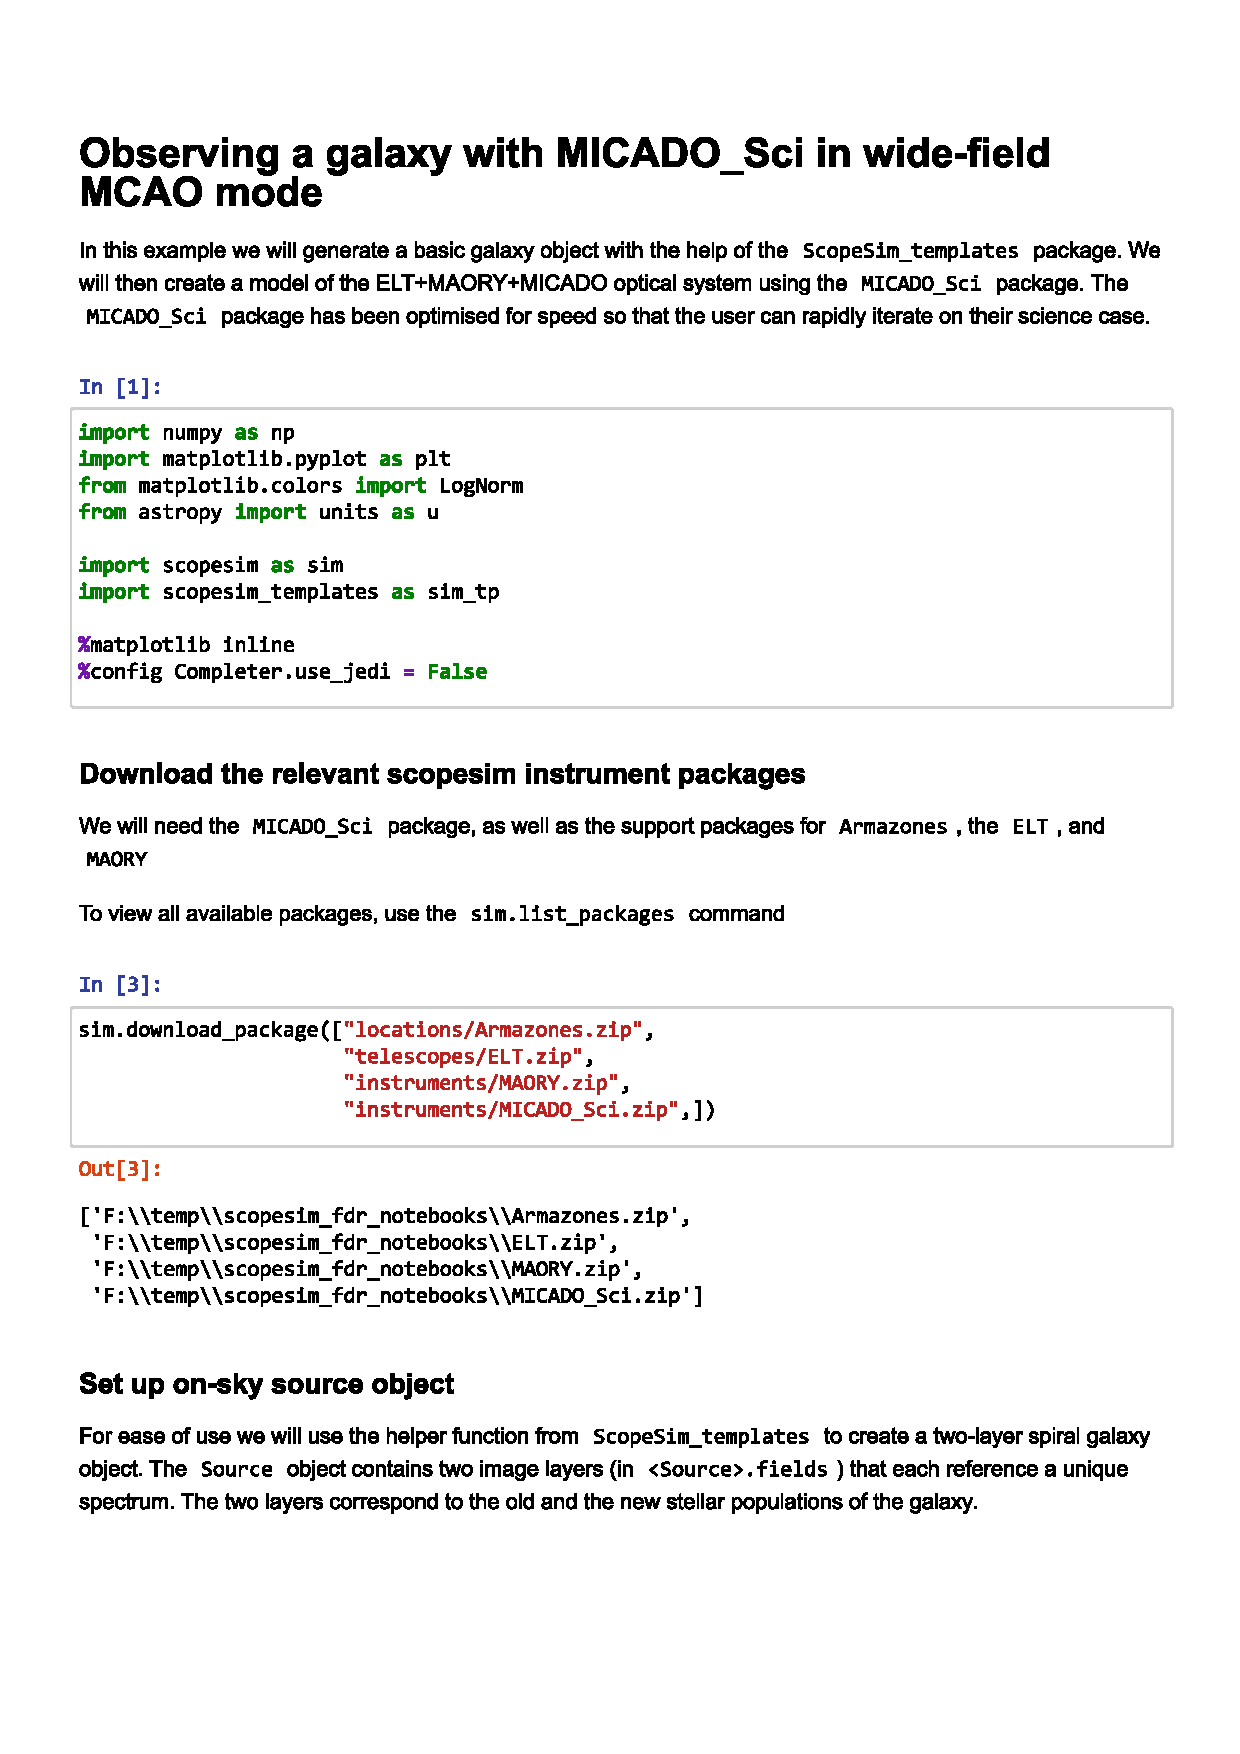
\includepdf[pages=-, scale=0.80]{tex/A_galaxy_with_micado_sci_mcao_4mas.pdf}

\stepcounter{subsection}
\addcontentsline{toc}{subsection}{\protect\numberline{\thesubsection}B: Astrometric observations of star cluster with SCAO, IMG\_1.5mas, and MICADO\_Sci}
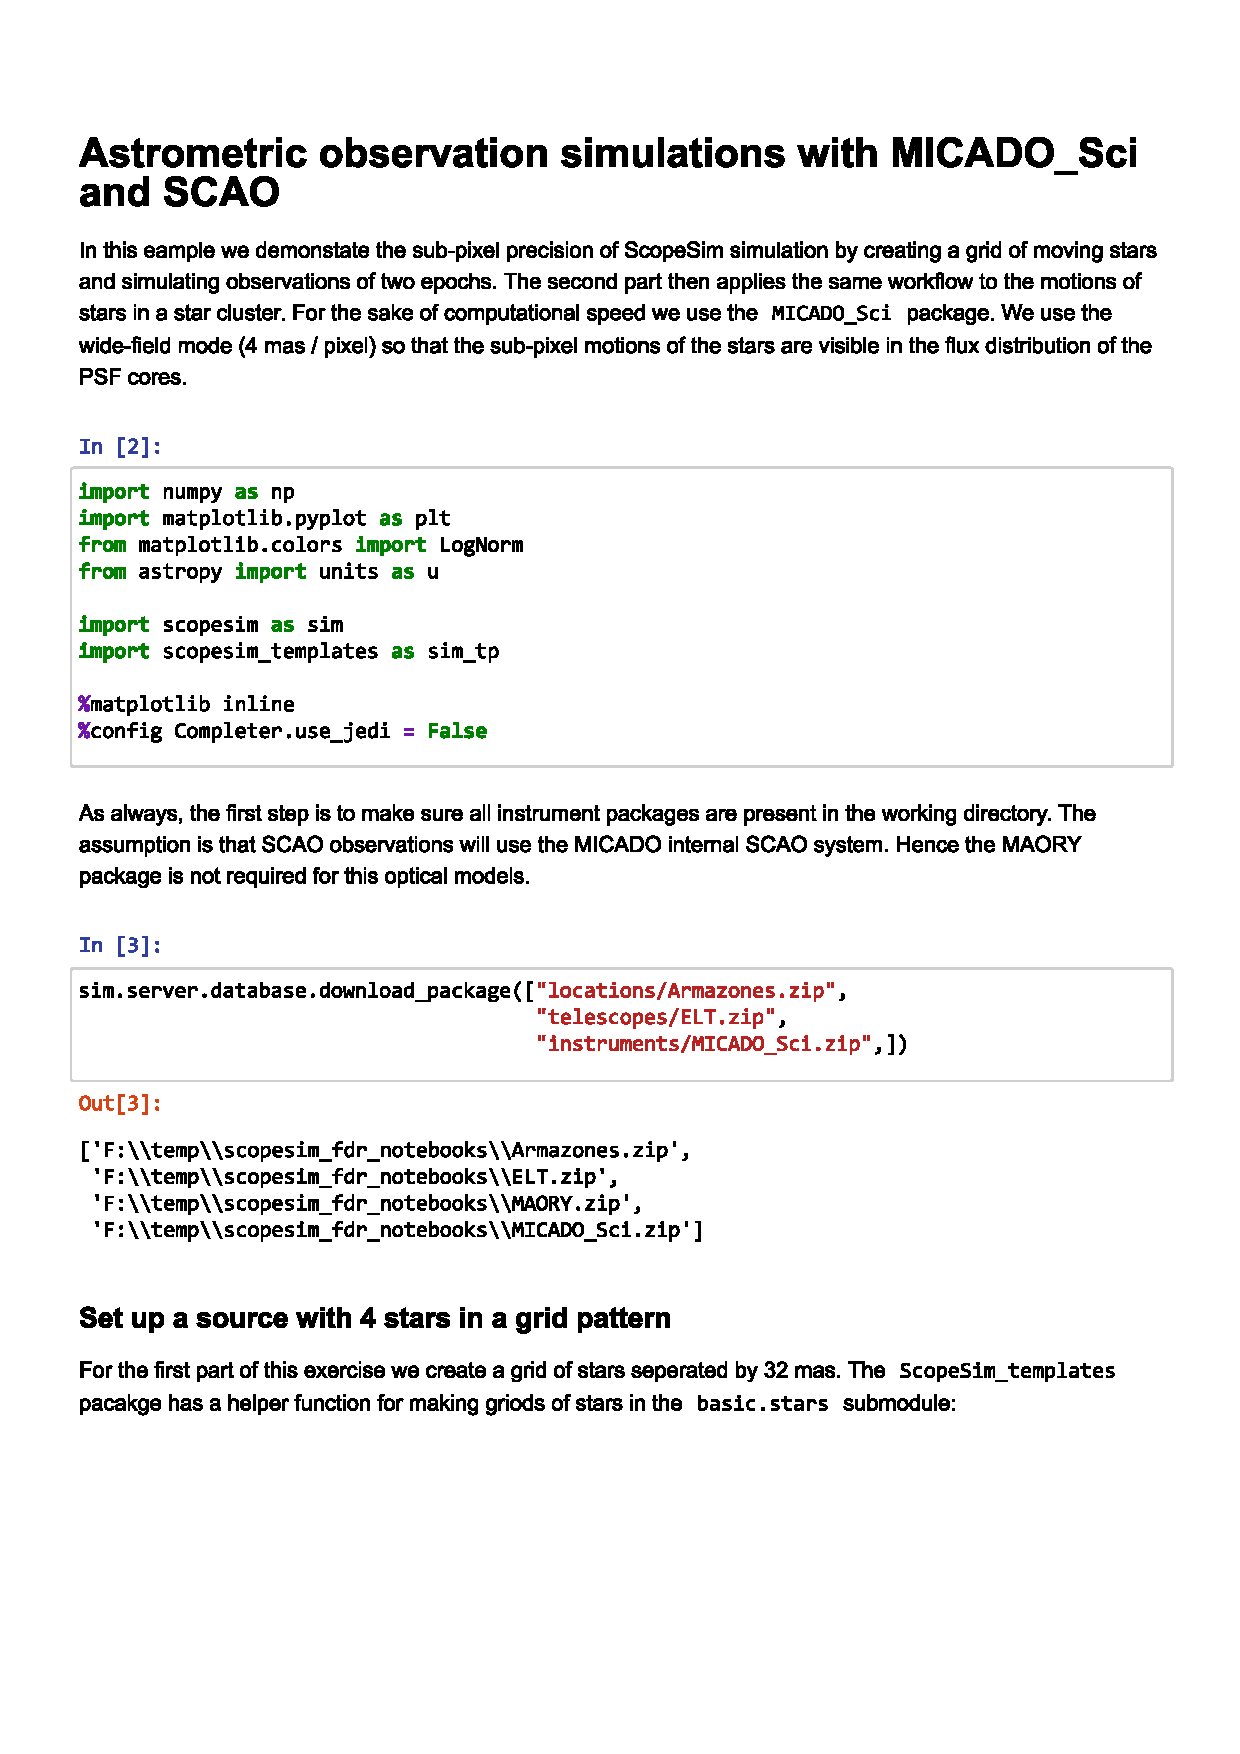
\includepdf[pages=-, scale=0.80]{tex/B_astrometry_with_micado_sci_scao_1_5mas.pdf}

\stepcounter{subsection}
\addcontentsline{toc}{subsection}{\protect\numberline{\thesubsection}C: PSF field variations with SCAO, variable pixel scales, and MICADO}
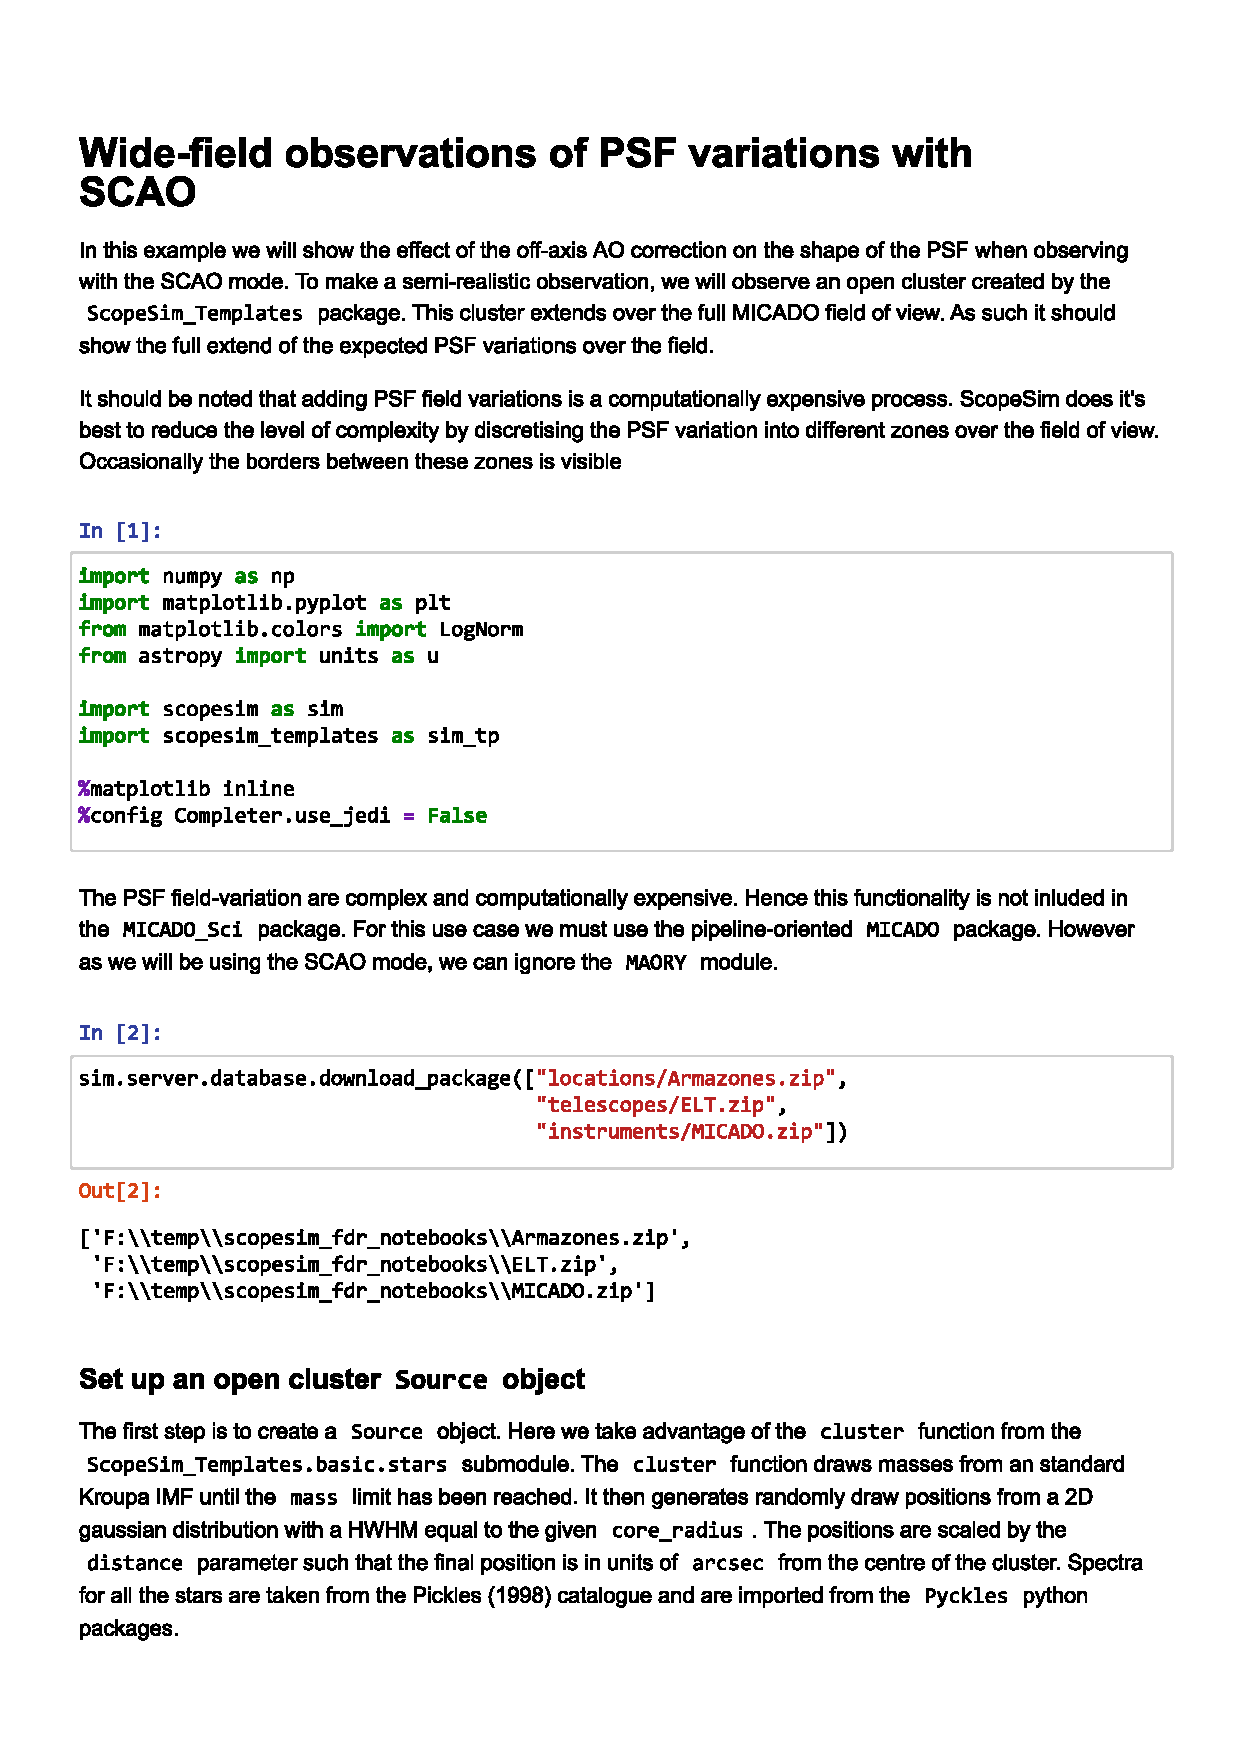
\includepdf[pages=-, scale=0.80]{tex/C_psf_field_variations_with_micado_pipe_scao.pdf}

\stepcounter{subsection}
\addcontentsline{toc}{subsection}{\protect\numberline{\thesubsection}D: Basic spectroscopy of galaxy core with variable slit size and MICADO\_Sci}
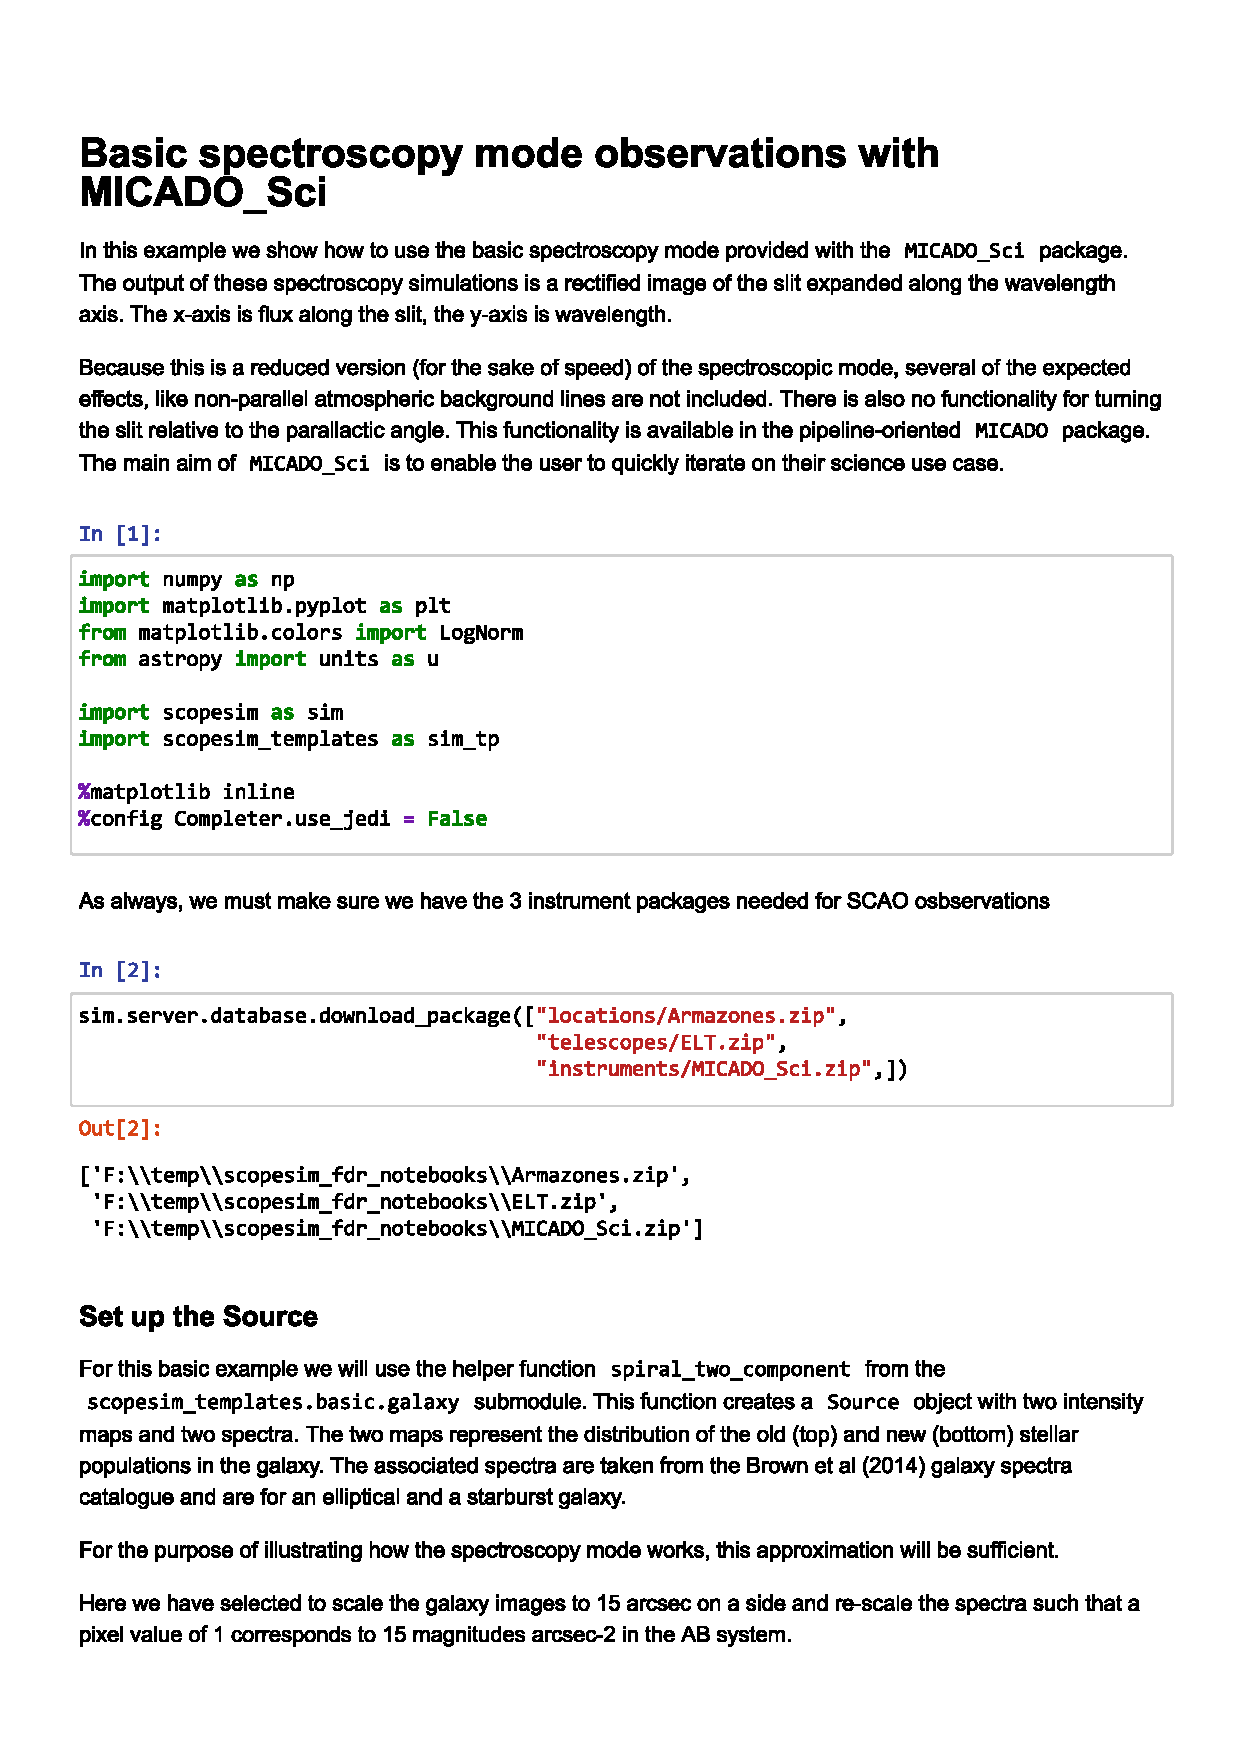
\includepdf[pages=-, scale=0.80]{tex/D_basioc_spectroscopy_with_micado_sci_spec.pdf}

\stepcounter{subsection}
\addcontentsline{toc}{subsection}{\protect\numberline{\thesubsection}E: Spectroscopy of binary stars with Spec\_HK, 3000x50 slit, and MICADO}
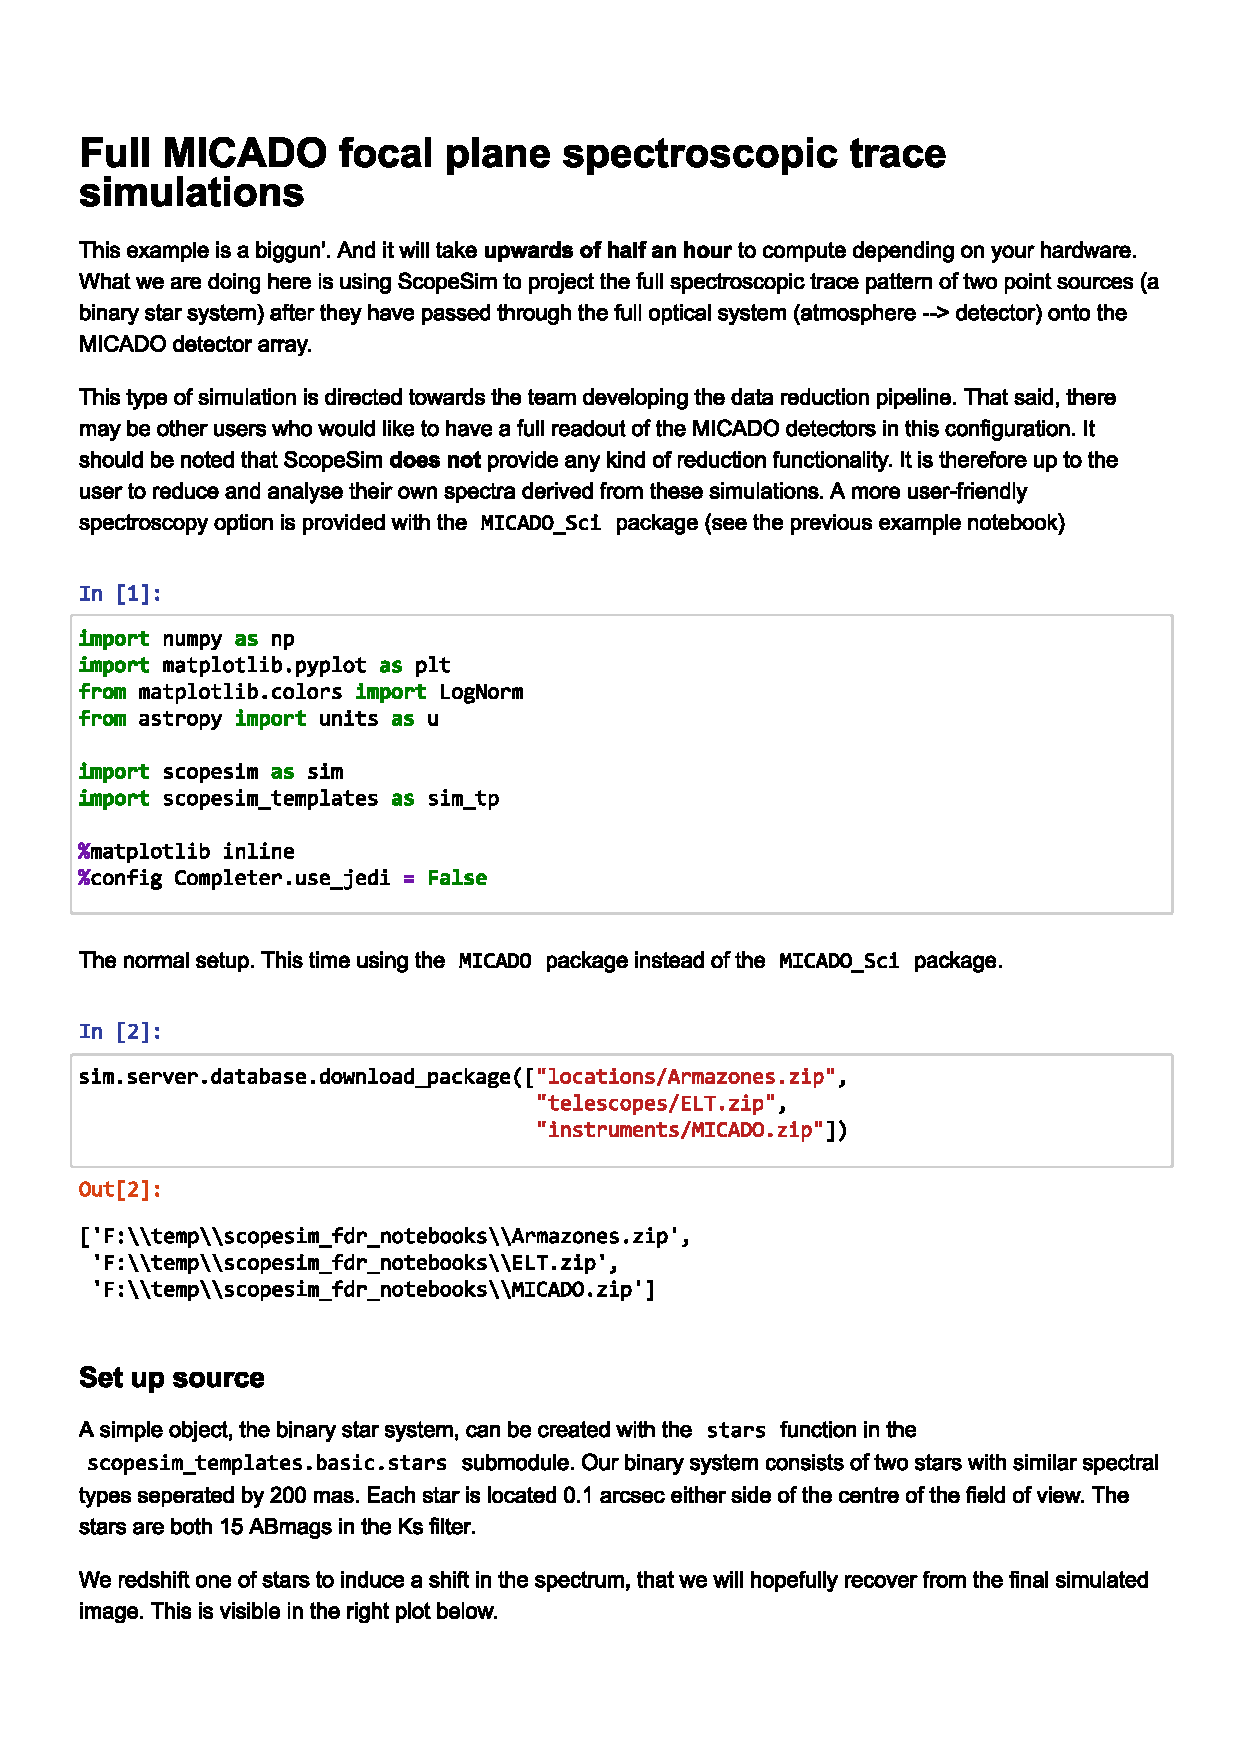
\includepdf[pages=-, scale=0.80]{tex/E_full_spectroscopy_pattern_with_micado_spec_3000x50.pdf}

\vspace*{\fill}
\centering
The previous page was unintentionally left blank.
\vspace*{\fill}

\end{document}
